\chapter{Forskningsmetoder og forskningsdesign}
\label{ch:method}

I dette kapittelet presenteres og drøftes forskningsmetodene og forskningsdesignet til studien.
I tillegg diskuteres validiteten til forskningen. 
Som skrevet tidligere, bygger forskningsprosessen på boken «Researching Information Systems and Computing» \citep{oates} (se figur \ref{fig:oates_model}).

\iffalse
I en forskningsartikkel er avsnittet om metode ofte det viktigste. Det samme gjelder metodekapitlet i en empirisk oppgave. Dette kan også være et vanskelig kapittel å skrive, fordi det ikke alltid er klart hvilken «jobb» det skal gjøre. Et metodekapittel skal ikke gjengi innholdet i fagets metodebøker. Dersom du har brukt intervju er det for eksempel ikke nødvendig å liste opp forskjellige typer forskningsintervju. Du trenger heller ikke redegjøre for forskjellene mellom kvantitative og kvalitative metoder, eller liste opp ulike typer validitet og reliabilitet.

Det du skal gjøre, er å vise hvordan dine valg av design og metode egner seg til å belyse/besvare ditt forskningsspørsmål, og hvilke vurderinger du har foretatt mht validitet (gyldighet) og reliabilitet (pålitelighet).’Show, don’t tell’ – vis leseren hva du gjorde, og forklar hvorfor. Da vil metodekapitlet sette de ulike delene av oppgaven i sammenheng, og det blir spennende å lese. I praksis betyr dette å demonstrere at du har forstått den praktiske betydningen av begrepene.

Et godt metodekapittel forteller hva du har gjort i din undersøkelse, og forklarer hvorfor. Hvordan samlet du inn data? Hva kan man forvente å finne ved å gjøre det på denne måten?
Hva var rammene? Hvilke avveininger måtte tas? Hva oppnår du ved å bruke denne metoden?
Vis hva du har gjort for å øke validiteten. Hva kan du si om reliabiliteten (påliteligheten) i datainnsamlingen? Hvordan vet du at du har undersøkt det du ønsket å undersøke? Hvilke slutninger kan trekkes på dette grunnlaget? Hvilke slutninger er sikre, og hvilke er mer tentative? Hvilken overføringsverdi har resultatene? Kan du generalisere – hvorfor, hvorfor ikke?
Svakheter og styrker ved metoden skal beskrives. Den ekstra gode oppgaven utmerker seg ved å forsvare sine valg og samtidig kritisere dem.

Formål
Produkter (bidrag/resultater)
Prosess
Deltakere
Paradigme
Presentasjon
\fi

%[width=0.85\textwidth,center]
\begin{figure}
\centering
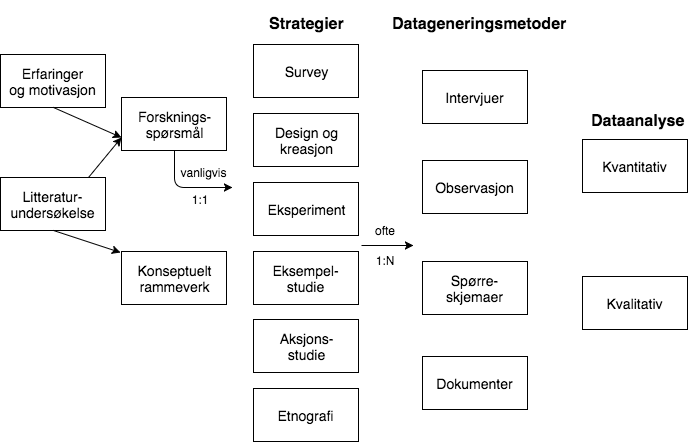
\includegraphics[width=\textwidth]{fig/oates/oates_research_norwegian}
\caption{Modell av forskningsprosessen fra \citet{oates}.}
\label{fig:oates_model}
\end{figure}

\section{Forskningsstrategier}
Som skrevet i kapittel \ref{ch:introduction}, er formålet med denne forskningen å undersøke hvordan ny teknologi basert
på \gls{iot}-skyløsninger kan brukes til avstandsoppfølging med prosjektet til Trondheim kommune som ramme. Dermed er å lage noe nytt,
«design og kreasjon», en naturlig hovedstrategi. Den støttende understrategien er en eksempelstudie av Trondheim kommunes arbeid
med avstandsoppfølging. De to strategiene er kort drøftet under.

\subsection{Design og kreasjon av et pulsoksimeter}
\textquote[\cite{oates}]{Forskningsmetoden design og kreasjon fokuserer på utvikling av nye IT-produkter, også kalt \textit{artefakter}.
Typer IT-artifakter inkluderer (March \& Smith, 1995): begreper, modeller, metoder og implementasjoner (engelsk: instantiations)}{.}

I følge \citet[s.121-122]{oates} er fordelene til denne strategien at det er enklere å relatere til noe som eksisterer i virkeligheten enn en íde, en tanke eller et konsept.
Den raske teknologiutviklingen gjør også at det er mulig å foreslå og utvikle nye artefakter, og at man dermed bidrar til ny kunnskap.

Ulempen med å velge denne strategien er at det er fort gjort at en kun demonstrerer
teknisk kompetanse uten at det kvalifiserer som god forskning. I tillegg til det nye produktet må ny kunnskap utvikles, bygget på analyse, argumenter
og kritiske evalueringer \citep[s. 109]{oates}. En ting er at det lages en prototype av et nytt produkt i et domene -- viktigere momenter er hvilken ny informasjon den fører
til og konteksten den blir satt inn i.

Brukersentrert utvikling er metodikken som brukes til designet og kreasjonen av prototypen. Det er en prosess der brukeren er involvert i hvert steg.
Stegene er å forstå brukskonteksten, etablere krav, implementere artefakt og evaluere artefakt. Dette er en syklus som kan gjentas flere ganger (se figur xxx).
Målet er å gjøre to iterasjoner av syklusen for å få mest mulig ut av metoden. Filosofien bak å inkludere brukeren i hvert aspekt av utviklingen er å fortere
finne ut hva som ikke fungerer slik at en ikke maler seg inn i et hjørne. Noe om ISO blabla. Eksempelstudien av avstandsoppfølging i Trondheim kommune vil
hjelpe til med å forstå konteksten pulsoksimeteret skal brukes i og hvordan det skal brukes, noe som vil føre til at utviklingen av en prototype blir enklere.

Noe om hvordan evalueringen skal foregå: intervju og observasjon


\subsection{Eksempelstudie: Avstandsoppfølging i Trondheim kommune}
\blindtext

\section{Forskningsspørsmål}
\subsection{Forskningsspørmål 1}
\textbf{Hvordan gjøres avstandsoppfølging av kronisk syke i dag, og hvilke planer finnes for ny teknologi på dette området?}

\subsection{Forskningsspørmål 2}
\textbf{Hva er en mulig teknologistakk for realisering av skybasert \gls{iot} for avstandsoppfølging av kronisk syke,
    [og hvordan skiller dette/denne seg fra eksisterende og planlagte løsninger]?}
    
\subsection{Forskningsspørmål 3}
\textbf{Hvordan vurderer domeneeksperter innen velferdsteknologi frittstående skybaserte \gls{iot}-løsninger for avstandsoppfølging av kronisk syke?}
 
\subsection{Forskningsspørmål 4}
\textbf{Basert på funnene fra FS1, FS2 og FS3, hva er implikasjonene for utviklingen av skybasert \gls{iot} som teknologisk plattform
    for avstandsoppfølging av kronisk syke?}

\section{Forskningsdesign}
\blindtext

\section{Validitet}

\section{Forskningsparadigme}